\documentclass[aspectratio=169, handout]{beamer}

% PACKAGES -----------------------------------------------------------------------------------------

\usepackage{array}
\usepackage{booktabs}
\usepackage{hyperref}
\usepackage{multirow}
\usepackage{ragged2e}
\usepackage{pgfplots}
\usepackage[dvipsnames]{xcolor}

\usetikzlibrary{arrows.meta, positioning, shadows}
\usepgfplotslibrary{groupplots}

% PLOT HELPERS -------------------------------------------------------------------------------------

% Process statistics for plots
\immediate\write18{data/statistics.sh}

% THEMING ------------------------------------------------------------------------------------------

% Beamer slide structure
\usetheme{Madrid}
\setbeamertemplate{navigation symbols}{}

% Beamer colors
\usecolortheme{beaver}
\setbeamercolor{item}{fg = darkred}
\setbeamercolor{section in head/foot}{bg = white}

% Beamer header
\addtobeamertemplate{frametitle}{\vspace{-0.2ex}}{\vspace{0.5ex}}
\setbeamercolor{frametitle}{fg = darkred, bg =}

% Beamer footer
\setbeamercolor{footer}{bg = white, fg = black}
\setbeamertemplate{footline}{
    \hbox{%
        \begin{beamercolorbox}[wd = .333333\paperwidth, ht = 2.25ex, dp = 1ex, left]{footer}
            \hspace{2ex}\insertshortauthor
        \end{beamercolorbox}%
        \begin{beamercolorbox}[wd = .333333\paperwidth, ht = 2.25ex, dp = 1ex, center]{footer}
            \insertshorttitle
        \end{beamercolorbox}%
        \begin{beamercolorbox}[wd = .333333\paperwidth, ht = 2.25ex, dp = 1ex, right]{footer}
            \insertframenumber\hspace{2ex}
        \end{beamercolorbox}
    }
}

% Other
\def\arraystretch{1.5}

% DOCUMENT INFORMATION -----------------------------------------------------------------------------

\title
    [Large Scale Hybrid Computing 25/26]
    {\large Tuning and Profiling LAMMPS on Deucalion}
\subtitle{\color{black} \small Large Scale Hybrid Computing 25/26}

\author[Group 2]{
    \begin{tabular}{lc}
        Humberto Gomes & \color{gray} pg59806 \\
        José Lopes     & \color{gray} pg59807
    \end{tabular}
}

\institute{
    Department of Informatics -- School of Engineering -- University of Minho \\
    \vspace{0.5\baselineskip}
    
\includegraphics[height=1cm]{res/SchoolOfEngineeringCropped.pdf}
}
\date{\scriptsize June 16\textsuperscript{th} 2026}

\newif\ifplacelogo
\logo{
    \ifplacelogo
        \begin{tikzpicture}[overlay, remember picture]
        \node[anchor = north east, inner sep = 0] at (current page.north east) {
            \LARGE
            
\includegraphics[height=1.1\baselineskip]{res/SchoolOfEngineeringCropped.pdf}
        };
        \end{tikzpicture}
    \fi
}

% PLOT HELPERS -------------------------------------------------------------------------------------

% Process statistics for plots
\immediate\write18{data/statistics.sh}

% DOCUMENT CONTENTS --------------------------------------------------------------------------------

\begin{document}

\placelogofalse
\frame[plain]{\titlepage}
\placelogotrue

\setcounter{framenumber}{0}
\justifying

\section{Introduction}

\begin{frame}{Introduction}
    \begin{itemize}
        \item Scientific simulations require ever more computation power;
        \item HPC systems offer substantial performance potential;
        \item LAMMPS is widely used for performing Molecular Dynamics simulations.
    \end{itemize}

    \vspace{\baselineskip}

    \begin{center}
        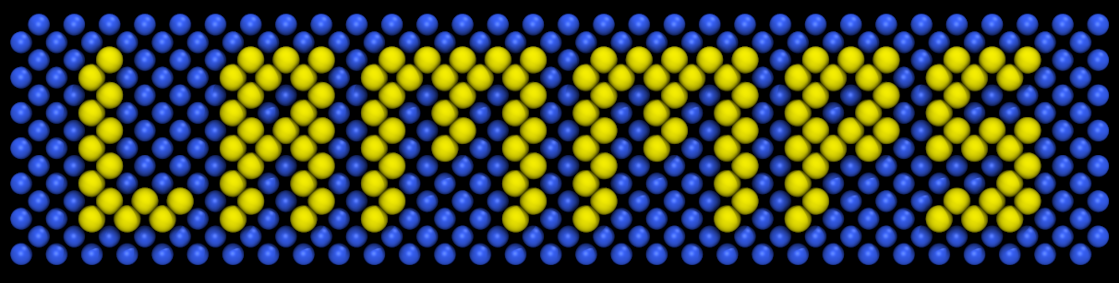
\includegraphics[width=0.6\textwidth]{res/LAMMPS.png} \\
        \small LAMMPS (Sandia Corporation)
    \end{center}
\end{frame}

\section{Background}

\begin{frame}{Background}
    \centering
    \begin{minipage}[t]{0.49\textwidth}
        \centering
        \textbf{LAMMPS} \\

        \vspace{\baselineskip}
        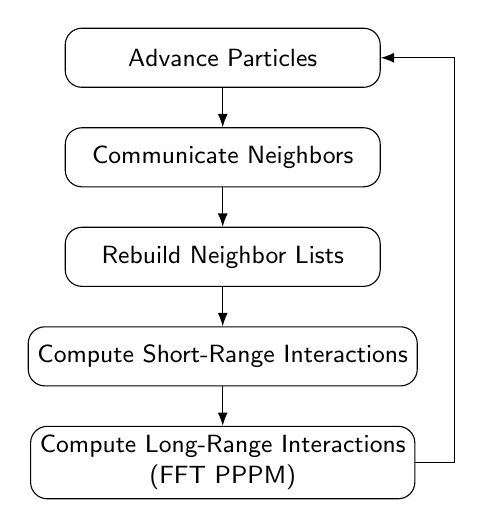
\begin{tikzpicture}[
            node distance  = 0.5cm,
            stepbox/.style = {
                rectangle,
                rounded corners = 6pt,
                draw            = black,
                fill            = white,
                align           = center,
                font            = \sffamily\small,
                minimum width   = 4cm,
                minimum height  = 0.75cm
            },
            flow/.style = {-{Latex}}
        ]

            \node[stepbox]                     (advance) {Advance Particles};
            \node[stepbox, below = of advance] (comm)    {Communicate Neighbors};
            \node[stepbox, below = of comm]    (build)   {Rebuild Neighbor Lists};
            \node[stepbox, below = of build]   (short)   {Compute Short-Range Interactions};
            \node[stepbox, below = of short]   (long)    {
                Compute Long-Range Interactions \\ (FFT PPPM)
            };

            \draw[flow] (advance) -- (comm);
            \draw[flow] (comm)    -- (build);
            \draw[flow] (build)   -- (short);
            \draw[flow] (short)   -- (long);
            \draw[flow]
                (long.east) -- ++(0.5,0)
                |- ([xshift=0.5cm]advance.east)
                -- (advance.east);
        \end{tikzpicture}
    \end{minipage}
    \begin{minipage}[t]{0.49\textwidth}
        \centering
        \textbf{Deucalion ARM Partition}
        \vspace{0.5\baselineskip}

        \begin{itemize}
            \item 48-core Fujitsu A64FX with NUMA;
        \end{itemize}

        \vspace{0.5\baselineskip}
        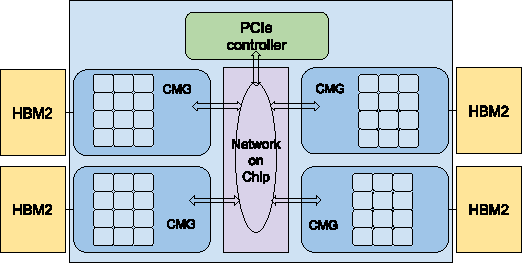
\includegraphics[width=0.95\textwidth]{res/A64FX.pdf}
        \vspace{0.5\baselineskip}

        \begin{itemize}
            \item Infiniband and Ethernet interconnects;
            \item LustreFS Parallel File System (PFS).
        \end{itemize}
    \end{minipage}
\end{frame}

\section{Benchmarks and Tuning Methodology}

\begin{frame}{Benchmarks and Tuning Methodology}

    \begin{itemize}
        \item Benchmarks with distinct computation characteristics:
        \begin{itemize}
            \item \textbf{LJ}: short-range interactions only, compute-bound;
            \item \textbf{Rhodo}: short and long range interactions, communication-sensitive.
        \end{itemize}
        \vspace{0.5\baselineskip}
        \item Cascading optimization with scalability analyses:
    \end{itemize}

    \begin{center}
        \resizebox{0.95\textwidth}{!}{
            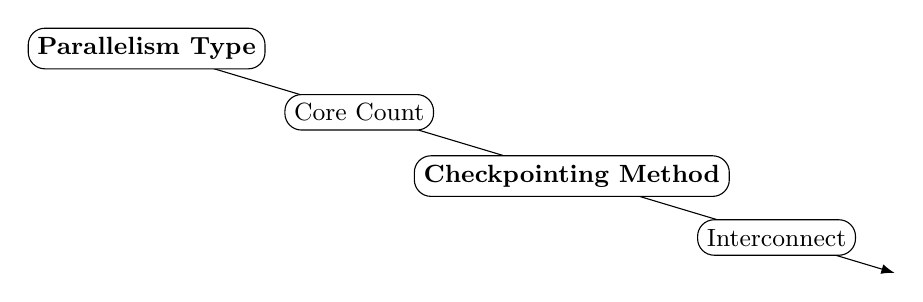
\begin{tikzpicture}[
                stepbox/.style = {
                    rectangle,
                    rounded corners = 6pt,
                    draw            = black,
                    fill            = white,
                    align           = center,
                    font            = \small
                },
                bigarrow/.style = {-{Latex}}
            ]

                \draw[bigarrow] (0, 0) -- (10, -3);
                \node[stepbox] at (0.5, -0.15) {\textbf{Parallelism Type}};
                \node[stepbox] at (3.2, -0.96) {Core Count};
                \node[stepbox] at (5.9, -1.77) {\textbf{Checkpointing Method}};
                \node[stepbox] at (8.5, -2.55) {Interconnect};
            \end{tikzpicture}
        }
    \end{center}
\end{frame}

\section{Tuning}

\begin{frame}{Tuning -- Parallelism Type}
    \begin{center}
        \resizebox{0.95\textwidth}{!}{\begin{tikzpicture}
    \begin{groupplot}[
        % Group two plots horizontally
        group style = {
            group size     = 2 by 1,
            horizontal sep = 1.6cm
        },
        % Plot dimensions
        width  = 0.48\textwidth,
        height = 5cm,
        % Axes styling
        xlabel             = {\# Nodes},
        x tick label style = {font = \scriptsize},
        y tick label style = {font = \scriptsize},
        xlabel near ticks,
        ylabel near ticks,
        x label style = {font = \small},
        y label style = {font = \small, align = center},
        % X axis range (shared)
        xmin = 0,
        xmax = 33,
        % Grid
        xtick       = {1, 2, 4, 8, 16, 32},
        xmajorgrids = true,
        ymajorgrids = true,
        grid style  = {dashed, gray!80}
    ]

        % ===== Left panel: LJ =====
        \nextgroupplot [
            ylabel = {\textbf{LJ} \\ \footnotesize Throughput (it/s)},
            ymin   = 0,
            ymax   = 9.99,
            ytick  = {0, 2, 4, 6, 8, 10},
            % Legend definition
            legend to name    = parallelism,
            legend cell align = left,
            legend style      = {
                legend columns                        = 6,
                font                                  = \small\ttfamily,
                /tikz/every even column/.append style = {column sep = 1ex}
            }
        ]

        \addplot+ [thick, red!80!black, mark = x, mark size = 2.5pt]
            table [x = NNODES, y = THROUGHPUT, col sep = comma] {data/parallelism/LJ-OMP-NUMA.csv};

        \addplot+ [thick, orange!80!black, mark = +, mark size = 2.5pt]
            table [x = NNODES, y = THROUGHPUT, col sep = comma] {data/parallelism/LJ-MPI.csv};

        \addplot+ [thick, ForestGreen, mark = |, mark size = 2.5pt]
            table [x = NNODES, y = THROUGHPUT, col sep = comma] {data/parallelism/LJ-KOKKOS-NUMA.csv};

        \addplot+ [thick, blue!80!black, mark = star, mark size = 2.5pt]
            table [x = NNODES, y = THROUGHPUT, col sep = comma] {data/parallelism/LJ-OMP.csv};

        \addplot+ [thick, black, mark = Mercedes star, mark size = 2.5pt]
            table [x = NNODES, y = THROUGHPUT, col sep = comma] {data/parallelism/LJ-KOKKOS.csv};

        \addplot+ [mark = none, black, thick, dotted] coordinates {(1, 0.275) (32, 8.8)};

        \legend{OMP-NUMA, MPI, KOKKOS-NUMA, OMP, KOKKOS, \textnormal{Linear}};

        % ===== Right panel: Rhodo =====
        \nextgroupplot [
            ylabel = {\textbf{Rhodo} \\ \footnotesize Throughput (it/s)},
            ymin   = 0,
            ymax   = 9.99,
            ytick  = {0, 2, 4, 6, 8, 10}
        ]

        \addplot+ [thick, red!80!black, mark = x, mark size = 2.5pt]
            table [x = NNODES, y = THROUGHPUT, col sep = comma] {data/parallelism/RHODO-OMP-NUMA.csv};

        \addplot+ [thick, orange!80!black, mark = +, mark size = 2.5pt]
            table [x = NNODES, y = THROUGHPUT, col sep = comma] {data/parallelism/RHODO-MPI.csv};

        \addplot+ [thick, blue!80!black, mark = star, mark size = 2.5pt]
            table [x = NNODES, y = THROUGHPUT, col sep = comma] {data/parallelism/RHODO-OMP.csv};

        \addplot+ [mark = none, black, thick, dotted] coordinates {(1, 0.275) (32, 10.24)};

    \end{groupplot}

    % Centered legend above both panels
    \path (group c1r1.north) -- (group c2r1.north)
        node[midway, anchor = south, yshift = 6pt] {
            \pgfplotslegendfromname{parallelism}
        };
\end{tikzpicture}
}
    \end{center}

    \begin{itemize}
        \item Linear scaling in LJ, but not Rhodo;
        \item Consistently better performance with \texttt{OMP-NUMA} (up to 10.8\% gains).
    \end{itemize}
\end{frame}

\begin{frame}{Tuning -- Checkpointing Strategy}
    \begin{itemize}
        \item Full simulation checkpoint every 100 iterations;
    \end{itemize}

    \begin{center}
        \resizebox{0.95\textwidth}{!}{\begin{tikzpicture}
    \begin{axis}[
        % Plot dimensions
        width  = 0.95\columnwidth,
        height = 4.2cm,
        % Axes styling
        xlabel             = {\# Nodes},
        x tick label style = {font = \scriptsize},
        y tick label style = {font = \scriptsize},
        xlabel near ticks,
        ylabel near ticks,
        % Label styles
        y label style = {font = \small, align = center},
        % Y axis
        ylabel = {\textbf{LJ} \\ \footnotesize Rel. throughput},
        ymin   = 0.81,
        ymax   = 1.05,
        % X axis range
        xmin = 0,
        xmax = 33,
        % Grid
        xtick       = {1, 2, 4, 8, 16, 32},
        xmajorgrids = true,
        ymajorgrids = true,
        grid style  = {
            dashed,
            gray!80
        },
        % Legend above the plot
        legend style = {
            at                                    = {(0.5, 1.03)},
            anchor                                = south,
            legend columns                        = 4,
            /tikz/every even column/.append style = {column sep = 0.5cm},
            font                                  = \footnotesize
        }
    ]

        \addplot+ [mark = none, black, very thick] coordinates {(1, 1) (32, 1)};

        \addplot+ [
            thick,
            red!80!black,
            mark      = x,
            mark size = 2.5pt
        ] table [
            x       = NNODES,
            y       = REL_THROUGHPUT,
            col sep = comma
        ] {data/storage/LJ-LOCAL.csv};

        \addplot+ [
            thick,
            ForestGreen,
            mark      = +,
            mark size = 2.5pt
        ] table [
            x       = NNODES,
            y       = REL_THROUGHPUT,
            col sep = comma
        ] {data/storage/LJ-PFS-SHARDED.csv};

        \addplot+ [
            thick,
            blue!80!black,
            mark      = Mercedes star,
            mark size = 2.5pt
        ] table [
            x       = NNODES,
            y       = REL_THROUGHPUT,
            col sep = comma
        ] {data/storage/LJ-PFS-SINGLE.csv};

        \legend{NOSTORAGE, LOCAL, PFS-SHARDED, PFS-SINGLE};
    \end{axis}
\end{tikzpicture}}
    \end{center}

    \begin{itemize}
        \item Checkpointing without significant overhead is possible;
        \item Up to 13.0\% performance loss with \texttt{PFS-SINGLE} (mainly due to stragglers).
    \end{itemize}
\end{frame}

\section{Profiling}

\begin{frame}{Profiling -- Methodology and Overhead}
    \begin{itemize}
        \item Questions:
        \begin{itemize}
            \item Kernels with optimization potential (1-node profiling);
            \item MPI communication breakdown and load imbalance (1-node vs 32-nodes);
            \item \ldots
        \end{itemize}
        \item High profiling overhead:
    \end{itemize}

    \begin{center}
        \resizebox{0.95\textwidth}{!}{\begin{tikzpicture}
    \begin{groupplot}[
        % Group two plots
        group style = {
            group size     = 2 by 1,
            horizontal sep = 2cm
        },
        % Plot dimensions
        width  = 0.48\columnwidth,
        height = 4.2cm,
        % Axes styling
        xlabel             = {\# Nodes},
        x tick label style = {font = \scriptsize},
        y tick label style = {font = \scriptsize},
        xlabel near ticks,
        ylabel near ticks,
        x label style = {font = \small},
        y label style = {font = \small, align = center},
        % X axis range
        xmin = 0,
        xmax = 33,
        % Grid
        xtick       = {1, 2, 4, 8, 16, 32},
        xmajorgrids = true,
        ymajorgrids = true,
        grid style  = {
            dashed,
            gray!80
        }
    ]

        % Top panel
        \nextgroupplot [
            % Y axis
            ylabel = {\textbf{Total} \\ \footnotesize Relative runtime},
            ymin   = 0.5,
            ymax   = 4.6,
            % Legend
            legend to name    = parallelism,
            legend cell align = left,
            legend style      = {
                at                                    = {(0.5, 1.05)},
                anchor                                = south,
                legend columns                        = 2,
                font                                  = \small,
                /tikz/every even column/.append style = {column sep = 1ex}
            }
        ]

        \addplot+ [mark = none, black, very thick] coordinates {(1, 1) (32, 1)};

        \addplot+ [
            thick,
            red!80!black,
            mark      = +,
            mark size = 2.5pt
        ] table [
            x       = NNODES,
            y       = REL_ALL,
            col sep = comma
        ] {data/overhead.csv};

        \legend{Baseline, NSight};

        % Bottom panel
        \nextgroupplot [
            % Y axis
            ylabel = {\textbf{Long-distance} \\ \footnotesize Relative runtime},
            ymin   = 0.5,
            ymax   = 16.0
        ]

        \addplot+ [mark = none, black, very thick] coordinates {(1, 1) (32, 1)};

        \addplot+ [
            thick,
            red!80!black,
            mark      = +,
            mark size = 2.5pt
        ] table [
            x       = NNODES,
            y       = REL_KSPACE,
            col sep = comma
        ] {data/overhead.csv};
    \end{groupplot}

    \path (group c1r1.north) -- (group c2r1.north)
        node[midway, anchor = south, yshift = 6pt] {
            \pgfplotslegendfromname{parallelism}
        };
\end{tikzpicture}}
    \end{center}
\end{frame}

\begin{frame}{Profiling -- Optimization Potential}
    \vspace{0.5\baselineskip}

    \centering
    \begin{minipage}{0.54\textwidth}
        \small
        \centering
        \begin{tabular}{lr}
            \toprule
            \textbf{Symbol}                           & {\textbf{Self (\%)}} \\
            \midrule
            \texttt{PairLJCharmmCoulLongOMP::compute} &    \color{red} 62.51 \\
            \texttt{NPairBinOmp<...>::build}          &                14.71 \\
            \texttt{PPPMOMP::fieldforce\_ik}          &                 7.11 \\
            \texttt{PPPMOMP::make\_rho}               &                 2.39 \\
            \midrule
            Others                                    &                13.28 \\
            \bottomrule
        \end{tabular}

        \vspace{0.5\baselineskip}
        \small Single node Rhodo call breakdown
    \end{minipage}
    \begin{minipage}{0.44\textwidth}
        \small
        \centering
        \begin{tabular}{lr}
                \toprule
                \textbf{Module Name}        & {\textbf{CPU Time (\%)}} \\
                \midrule
                \texttt{liblammps.so.0}     &        \color{red} 96.87 \\
                \texttt{libm-2.28.so}       &                     1.53 \\
                \texttt{libgomp.so.1.0.0}   &                     0.51 \\
                \texttt{libfftw3.so.3.6.10} &        \color{blue} 0.44 \\
                \midrule
                Others                      &                     0.65 \\
                \bottomrule
        \end{tabular}

        \vspace{0.5\baselineskip}
        \small Single node Rhodo module breakdown
    \end{minipage}

    \vspace{\baselineskip}
    \begin{itemize}
        \item Dominant compute-bound kernel $\rightarrow$ compiler changes, SIMD implementation;
        \item Little opportunity for optimized external library.
    \end{itemize}
\end{frame}

\begin{frame}{Profiling -- MPI Communication Breakdown}
    \begin{center}
        \resizebox{0.8\textwidth}{!}{
            \begin{tabular}{lrr!{\vrule width 0.8 pt}rr}
                \toprule
                \multirow{2}{*}{\textbf{MPI Directive}}          &
                \multicolumn{2}{c!{\vrule width 0.8 pt}}{1-node} &
                \multicolumn{2}{c}{8-node}                       \\
                \cmidrule(lr){2-3} \cmidrule(lr){4-5}

                                        &
                \textbf{MPI Time  (\%)} &
                \textbf{Wall Time (\%)} &
                \textbf{MPI Time  (\%)} &
                \textbf{Wall Time (\%)} \\
                \midrule

                \texttt{MPI\_Wait}      & 41.0 & 1.32 &          41.0 & \textbf{7.69} \\
                \texttt{MPI\_Allreduce} & 31.0 & 1.01 &          28.0 & \textbf{5.30} \\
                \texttt{MPI\_Send}      & 21.0 & 0.68 &          16.0 & \textbf{2.98} \\
                \texttt{MPI\_Waitany}   &   -- &   -- &  \textbf{7.0} & \textbf{1.45} \\
                Others                  &  7.0 &   -- &           8.0 &   -- \\
                \bottomrule
            \end{tabular}
        }

        \vspace{0.5\baselineskip}
        \small MPI directive time on $1$-node and $8$-node configurations
    \end{center}

    \begin{itemize}
        \item Growth in communication time with node count (3.1\% $\rightarrow$ 17.7\%);
        \item Reported performance disparities of up to \textcolor{red}{25.1\%} between MPI ranks;
        \item Collective MPI directives, non-blocking MPI directives, \ldots
    \end{itemize}
\end{frame}

\section{Conclusion}

\begin{frame}{Conclusion}
    \begin{itemize}
        \item MPI+OpenMP NUMA-aware setup achieved performance improvements of 10.8\%;
        \item Sharding can eliminate the performance overhead of simulation checkpointing;
        \item Profiling revealed future work opportunities.
    \end{itemize}

    \begin{center}
        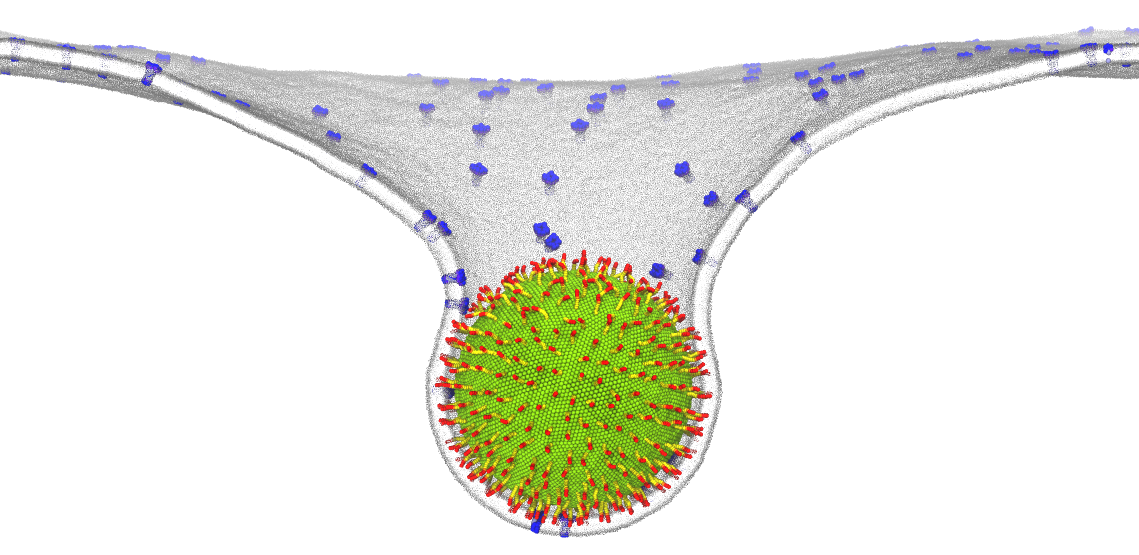
\includegraphics[width=0.6\textwidth]{res/LAMMPSSim.png} \\
        \small LAMMPS Simulation Visualization (Comp Phys Comm)
    \end{center}
\end{frame}

\placelogofalse
\frame[plain]{\titlepage}
\placelogotrue

\end{document}
